\documentclass{article}
\usepackage{graphicx} % Required for inserting images
\usepackage{lipsum}
\usepackage{bm}
\usepackage{stmaryrd}
\usepackage{tikz}
\usepackage{stanli}
\usepackage{amsmath}
\usetikzlibrary {arrows.meta,bending}
\usepackage{graphicx} % Required for inserting images



\title{Introduction di Finite Elements}
\author{Group 3}
\date{November 2023}

\begin{document}

\maketitle

\section{Weak form of ellipict equations}
\begin{equation}
    u''(x) = -f(x)    
\end{equation}





\section{Introduction}

\section{Formulation}
In Figure \ref{fig:1dTruss} an axially loaded linear elastic
truss is depicted with certain boundary conditions. For this case the ODE is shown in equation \ref{eq:1D_Truss} and the boundary conditions are in equation \ref{eq:BC_Truss}. 

\vspace{2ex}

\begin{figure}[h]
\centering
    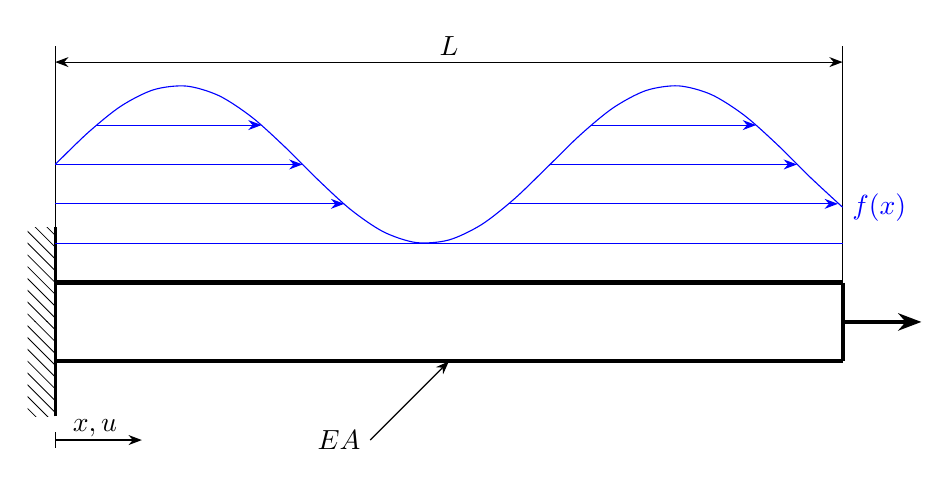
\begin{tikzpicture}[domain=0:10,smooth]
        %\draw[help lines,step =.5](-2 ,-2)grid(10 ,2);
        \point{a}{0}{0.6};
        \point{b}{0}{-0.6};
        \point{c}{0}{0.5};
        \point{d}{0}{-0.5};
        \point{e}{10}{0.5};
        \point{f}{10}{-0.5};
        \point{o}{0}{-1.5};
        \draw(0,-1.4)--(0,-1.6);
        \draw[-{Stealth}](0,-1.5)--(1.1,-1.5);
        \draw (0.1,-1.35) node[right] {$x,u$};
        %\node(0,0)node[left]{$x,u$};
        \support{3}{a}[270];
        \support{3}{b}[270];
        \beam{2}{c}{e};
        \beam{2}{e}{f};
        \beam{2}{f}{d};
        \draw(0,0)--(0,3.5);
        \draw(10,0)--(10,3.5);
        \draw [{Stealth}-{Stealth}](0,3.3)--(10,3.3);
        \draw (5,3.5) node[] {$L$};
        \draw[color=blue]   plot (\x,{sin(\x r)+2})    node[right] {$f(x)$};
        \draw[color=blue](0,1)--(10,1);
        \draw[color=blue,-{Stealth}](0,2)--(3.14,2);
        \draw[color=blue,-{Stealth}](6.28,2)--(9.42,2);
        \draw[color=blue,-{Stealth}](0,1.5)--(3.67,1.5);
        \draw[color=blue,-{Stealth}](5.76,1.5)--(9.94,1.5);
        \draw[color=blue,-{Stealth}](0.52,2.5)--(2.62,2.5);
        \draw[color=blue,-{Stealth}](6.81,2.5)--(8.9,2.5);
        \draw[very thick,-{Stealth}](10,0)--(11,0);
        \draw[{Stealth}-](5,-0.5)--(4,-1.5);
        \draw (4,-1.5) node[left] {$EA$};
    \end{tikzpicture}
    \caption{1D Truss}\label{fig:1dTruss}
\end{figure}




\vspace{2ex}

For this analysis, the properties of the truss remain constant. Additionally, the truss exhibits
a linear elastic stress–strain relationship.

\vspace{2ex}

\begin{equation}\label{eq:1D_Truss}
    EA\frac{d^2u}{dx^2} + f(x)=0
\end{equation}

\vspace{2ex}

\begin{equation}\label{eq:BC_Truss}
    \begin{gathered}
        u(0)=0\\
        EA\frac{du(L)}{dx}=F
    \end{gathered}
\end{equation}

\vspace{2ex}


\subsection{Discretization}

Initially the domain is discretized in $k$ elements, each of these elements has $n$ nodes. The displacement approximation is shown in equation \ref{eq:u_Truss}, where $\varphi_i$ are the shape functions and $u_i$ the displacement. 

\vspace{2ex}

%\begin{figure}[h]
%\centering
 %   \includegraphics[width=0.7\textwidth]{chapters/Truss/1D Truss D.png}
  %  \caption{1D Truss discrete domain}\label{fig:1dTrussD}
%\end{figure}




\begin{figure}[h]
\centering
    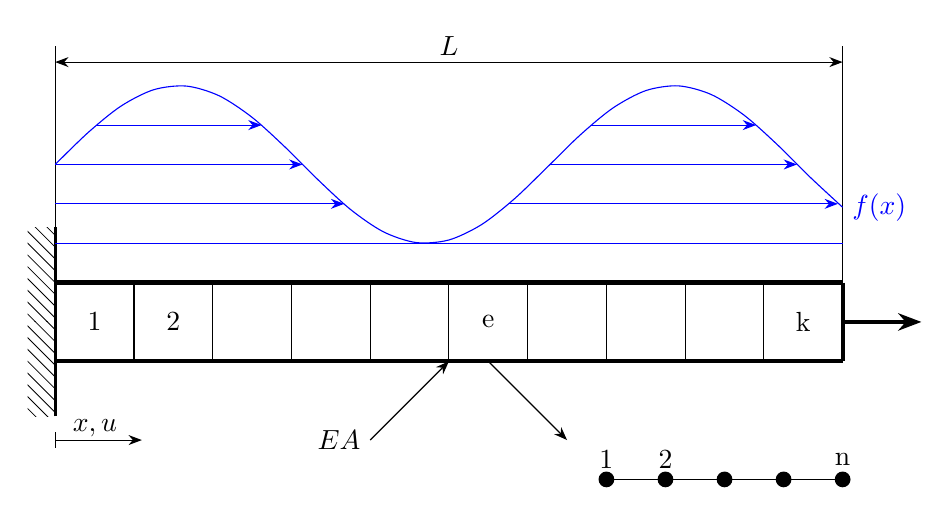
\begin{tikzpicture}[domain=0:10,smooth]
        \foreach \i in {1,...,9}
        {;
        \draw(\i,-0.5)--(\i,0.5);
        }
        \point{a}{0}{0.6};
        \point{b}{0}{-0.6};
        \point{c}{0}{0.5};
        \point{d}{0}{-0.5};
        \point{e}{10}{0.5};
        \point{f}{10}{-0.5};
        \point{o}{0}{-1.5};
        \draw(0,-1.4)--(0,-1.6);
        \draw[-{Stealth}](0,-1.5)--(1.1,-1.5);
        \draw (0.1,-1.35) node[right] {$x,u$};
        %\node(0,0)node[left]{$x,u$};
        \support{3}{a}[270];
        \support{3}{b}[270];
        \beam{2}{c}{e};
        \beam{2}{e}{f};
        \beam{2}{f}{d};
        \draw(0,0)--(0,3.5);
        \draw(10,0)--(10,3.5);
        \draw [{Stealth}-{Stealth}](0,3.3)--(10,3.3);
        \draw (5,3.5) node[] {$L$};
        \draw[color=blue]   plot (\x,{sin(\x r)+2})    node[right] {$f(x)$};
        \draw[color=blue](0,1)--(10,1);
        \draw[color=blue,-{Stealth}](0,2)--(3.14,2);
        \draw[color=blue,-{Stealth}](6.28,2)--(9.42,2);
        \draw[color=blue,-{Stealth}](0,1.5)--(3.67,1.5);
        \draw[color=blue,-{Stealth}](5.76,1.5)--(9.94,1.5);
        \draw[color=blue,-{Stealth}](0.52,2.5)--(2.62,2.5);
        \draw[color=blue,-{Stealth}](6.81,2.5)--(8.9,2.5);
        \draw[very thick,-{Stealth}](10,0)--(11,0);
        \draw[{Stealth}-](5,-0.5)--(4,-1.5);
        \draw (4,-1.5) node[left] {$EA$};
        \draw (0.5,0) node[] {1};
        \draw (1.5,0) node[] {2};
        \draw (5.5,0) node[] {e};
        \draw (9.5,0) node[] {k};
        \draw[-{Stealth},bend left](5.5,-0.5)--(6.5,-1.5);
        \foreach \i in {1,...,5}
        {;
        \fill (6.25+0.75*\i,-2) circle (0.1);
        }
        \draw (7,-2) --(10,-2);
        \draw (7,-1.75) node[] {1};
        \draw (7.75,-1.75) node[] {2};
        \draw (10,-1.75) node[] {n};
    \end{tikzpicture}
    \caption{1D Truss discrete domain}\label{fig:1dTrussD}
\end{figure}

\vspace{2ex}

\begin{equation}\label{eq:u_Truss}
    u^{(e)}\approx \tilde{u}=\sum_{i=1}^{n}{u_{i}\varphi_{i}}=[\varphi]^T[u]
\end{equation}

\vspace{2ex}

\begin{equation}\label{eq:vectors}
    \begin{gathered}
        \relax[u]=[u_1 \quad u_2 \quad ... \quad ... \quad u_n]^T\\
        \relax[\varphi]=[\varphi_1 \quad \varphi_2 \quad ... \quad ... \quad \varphi_n]^T\\
        \relax\left[\frac{d\varphi}{dx}\right]=\left[\frac{d\varphi_1}{dx} \quad \frac{d\varphi_2}{dx} \quad ... \quad ... \quad \frac{d\varphi_n}{dx}\right]^T\\
        \relax\left[\frac{d\varphi}{d\xi}\right]=\left[\frac{d\varphi_1}{d\xi} \quad \frac{d\varphi_2}{d\xi} \quad ... \quad ... \quad \frac{d\varphi_n}{d\xi}\right]^T\\
    \end{gathered}
\end{equation}

\vspace{2ex}

\section{Galerkin Method}

The Galerkin method formulation for each element is shown next: 

\vspace{2ex}

\begin{equation}\label{eq:GM_Formulation}
    \begin{gathered}
        R=EA\frac{d^2\tilde{u}}{dx^2}+f(x)\\
        \int_{x_e}^{x_e+h}{R\cdot v \cdot dx}=\int_{x_e}^{x_e+h}{\left(EA\frac{d^2\tilde{u}}{dx^2}+f(x) \right)\cdot[\varphi]\cdot dx}=0\\
        EA\left([\varphi]\frac{d\tilde{u}}{dx}\right)\Bigg\rvert_{x_e}^{x_e+h}-EA\int_{x_e}^{x_e+h}{\frac{d\tilde{u}}{dx}\cdot \left[\frac{d\varphi}{dx}\right] \cdot dx}+\int_{x_e}^{x_e+h}{f(x) \cdot[\varphi]\cdot dx}=0\\
        -EA\left([\varphi]\cdot\left[\frac{d\varphi}{dx}\right]^T\cdot [u]\right)\Bigg\rvert_{x_e}^{x_e+h}+\left(EA\int_{x_e}^{x_e+h}{ \left[\frac{d\varphi}{dx}\right] \cdot \left[\frac{d\varphi}{dx}\right]^T\cdot dx}\right) [u]=\int_{x_e}^{x_e+h}{f(x) \cdot[\varphi]\cdot dx} 
    \end{gathered}
\end{equation}

\vspace{2ex}

By taking into account the continuity between each of the elements, it can be observed that the first term of the equation is eliminated for all degrees of freedom when the system is assembled, except for the first and last ones. In these cases, the boundary conditions come into play, enabling the linear system to be solved. In Equation \ref{eq:GM_Truss_Local} the system of equations is transformed into natural coordinates, allowing an easy formulation for every element.

\vspace{2ex}

\begin{equation}\label{eq:GM_Truss_Local}
\begin{aligned}
    -EA\left([\varphi]\cdot\left[\frac{d\varphi}{d\xi}\right]^T \left(\frac{d\xi}{dx}\right)\cdot [u]\right)\Bigg\rvert_{-1}^{1}+\left(EA\int_{-1}^{1}{ \left[\frac{d\varphi}{d\xi}\right] \cdot \left[\frac{d\varphi}{d\xi}\right]^T\left(\frac{d\xi}{dx}\right)\cdot d\xi}\right) [u]\\
    =\int_{-1}^{1}{f\left(x(\xi)\right) \cdot[\varphi]\cdot \left(\frac{dx}{d\xi}\right) d\xi}
\end{aligned}
\end{equation}

\vspace{2ex}


\section{Formulation Beam}

Figure \ref{fig:1dBeam}  illustrates a 1D beam subjected to a distributed load $q(x)$ along its length. The problem formulation employs the Euler-Bernoulli beam theory (Equation \ref{eq:1D_Beam}, where $w(x)$ is the deflection). It is important to note that throughout this analysis, the properties of the beam remain constant. Furthermore, the material properties are assumed to demonstrate only linear elastic behavior.


\vspace{2ex}


\begin{figure}[h]
\centering
    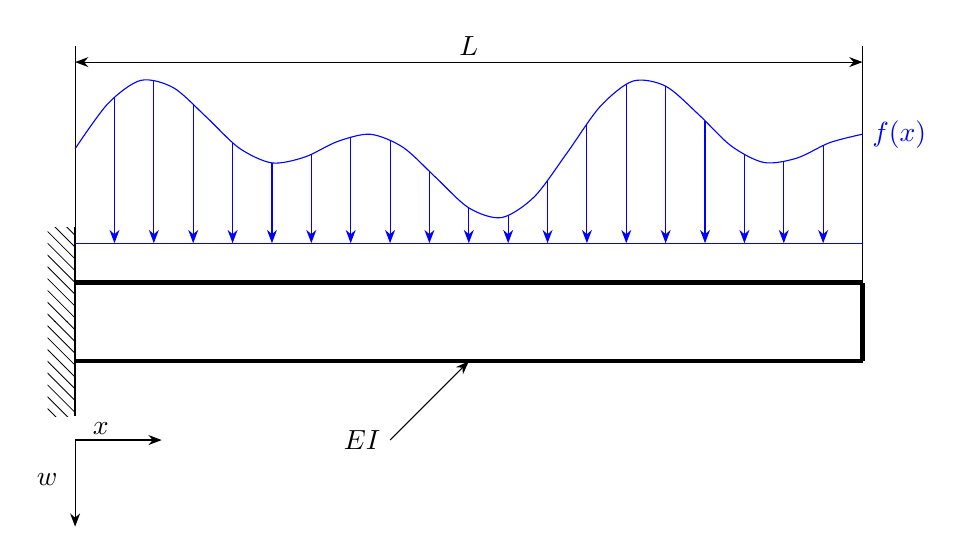
\begin{tikzpicture}[domain=0:10,smooth]
        %\draw[help lines,step =.5](-2 ,-2)grid(10 ,2);
        \point{a}{0}{0.6};
        \point{b}{0}{-0.6};
        \point{c}{0}{0.5};
        \point{d}{0}{-0.5};
        \point{e}{10}{0.5};
        \point{f}{10}{-0.5};
        \point{o}{0}{-1.5};
        \draw[-{Stealth}](0,-1.5)--(1.1,-1.5);
        \draw[-{Stealth}](0,-1.5)--(0,-2.6);
        \draw (0.1,-1.35) node[right] {$x$};
        \draw (-0.1,-2) node[left] {$w$};
        %\node(0,0)node[left]{$x,u$};
        \support{3}{a}[270];
        \support{3}{b}[270];
        \beam{2}{c}{e};
        \beam{2}{e}{f};
        \beam{2}{f}{d};
        \draw(0,0)--(0,3.5);
        \draw(10,0)--(10,3.5);
        \draw [{Stealth}-{Stealth}](0,3.3)--(10,3.3);
        \draw (5,3.5) node[] {$L$};
        \draw[color=blue]   plot (\x,{(sin(\x r)+sin(2*\x r))*0.5+2.2})    node[right] {$f(x)$};
        \foreach \i in {1,...,19}
        {
            \pgfmathsetmacro{\x}{(sin(0.5*\i r)+sin(\i r))*0.5+2.2}
            \draw[color=blue,-{Stealth}](0.5*\i,\x)--(0.5*\i,1);
        }
        \draw[color=blue](0,1)--(10,1);
        
        %\draw[color=blue,-{Stealth}](6.28,2)--(9.42,2);
        %\draw[color=blue,-{Stealth}](0,1.5)--(3.67,1.5);
        %\draw[color=blue,-{Stealth}](5.76,1.5)--(9.94,1.5);
        %\draw[color=blue,-{Stealth}](0.52,2.5)--(2.62,2.5);
        %\draw[color=blue,-{Stealth}](6.81,2.5)--(8.9,2.5);
        
        \draw[{Stealth}-](5,-0.5)--(4,-1.5);
        \draw (4,-1.5) node[left] {$EI$};
    \end{tikzpicture}
    \caption{1D Beam}\label{fig:1dBeam}
\end{figure}


\vspace{2ex}

\begin{equation}\label{eq:1D_Beam}
    EI\frac{d^4w}{dx^4}=q(x)
\end{equation}

\vspace{2ex}

The boundary conditions in this case are the deflection and slope, Equation (23). 

\begin{equation}\label{eq:BC_Beam}
    \begin{gathered}
        w(0)=0\\
        \frac{dw(0)}{dx}=0
    \end{gathered}
\end{equation}

\vspace{2ex}

Similar to the analysis conducted for the truss element, the objective of this study is to approximate the deflection $w$ and slope $\frac{dw}{dx}$ using two distinct approaches: the standard Galerkin Method and the Discontinuous Galerkin Method. 

\subsection{Discretization}

Initially the domain is discretized in $k$ elements, each of these elements has 2 nodes, and each of this nodes has two degrees of freedom. The deflection approximation is shown in Equation \ref{eq:w_Beam}, where $\varphi_i$ are the shape functions, $w_i$ the deflection and $\theta_i$ the slope. Additional relationships are in Equation \ref{eq:vectors_B}

\vspace{2ex}

\begin{equation}\label{eq:w_Beam}
    w^{(e)}\left(x\right)\approx\tilde{w}=\sum_{i=1}^{4}{w_i\varphi_i}=\left[\varphi\right]^T[w]
\end{equation}

\vspace{2ex}

\begin{equation}\label{eq:vectors_B}
    \begin{gathered}
        \left[w\right]=\left[\begin{matrix}w_1&\theta_1&w_2&\theta_2\\\end{matrix}\right]^T\\
       \left[M\right]=\left[\begin{matrix}M&V_1&M_2&V_2\\\end{matrix}\right]^T\\
       \left[\varphi\right]=\left[\begin{matrix}\varphi_1&\varphi_2&\varphi_3&\varphi_4\\\end{matrix}\right]^T\\
        \left[\frac{d\varphi}{dx}\right]=\left[\begin{matrix}\frac{d\varphi_1}{dx}&\frac{d\varphi_2}{dx}&\frac{d\varphi_3}{dx}&\frac{d\varphi_4}{dx}\\\end{matrix}\right]^T\\
        \left[\frac{d\varphi}{dx}\right]=\left[\begin{matrix}\frac{d\varphi_1}{d\xi}&\frac{d\varphi_2}{d\xi}&\frac{d\varphi_3}{d\xi}&\frac{d\varphi_4}{d\xi}\\\end{matrix}\right]^T\left(\frac{d\xi}{dx}\right)\\
        M^{(e)}\left(x\right)\approx\tilde{M}=\left[\varphi\ \right]^T\left[M\right]\\
        \frac{d\hat{w}}{dx}=\hat{\theta}\\
        \frac{d\hat{M}}{dx}=\hat{V}
    \end{gathered}
\end{equation}

The shape functions used in this case are the Hermitian polynomials, which are already proven to be a good choice for beam elements.

\section{Galerkin Method}

\begin{equation}\label{eq:GM_beam}
    \begin{gathered}
        R=EI\frac{d^4\widetilde{w}}{dx^4}-q\left(x\right)\\
        \int_{x_e}^{x_e+h}{R\cdot v\cdot d x}=\int_{x_e}^{x_e+h}{\left(EI\frac{d^4\widetilde{w}}{dx^4}-q\left(x\right)\right)\cdot\left[\varphi\right]\cdot dx}=0\\
        EI\left(\left[\varphi\right]\frac{d^3\widetilde{w}}{dx^3}\right)\Bigg\rvert_{x_e}^{x_e+h}-EI\left(\left[\frac{d\varphi}{dx}\right]\frac{d^2\widetilde{w}}{dx^2}\right)\Bigg\rvert_{x_e}^{x_e+h}+EI\int_{x_e}^{x_e+h}{\frac{d^2\widetilde{w}}{dx^2}\cdot\left[\frac{d^2\varphi}{dx^2}\right]\cdot d x}\\-\int_{x_e}^{x_e+h}{q\left(x\right)\cdot\left[\varphi\right]\cdot d x}=0\\
        EI\left(\left[\varphi\right]{\cdot\left[\frac{d^3\varphi}{dx^3}\right]}^T\cdot\left[w\right]\right)\Bigg\rvert_{x_e}^{x_e+h}-EI\left(\left[\frac{d\varphi}{dx}\right]{\cdot\left[\frac{d^2\varphi}{dx^2}\right]}^T\cdot\left[w\right]\right)\Bigg\rvert_{x_e}^{x_e+h}\\+EI\left(\int_{x_e}^{x_e+h}{\left[\frac{d^2\varphi}{dx^2}\right]{\cdot\left[\frac{d^2\varphi}{dx^2}\right]}^T\cdot d x}\right)\left[w\right]=\int_{x_e}^{x_e+h}{q\left(x\right)\cdot\left[\varphi\right]\cdot d x}
    \end{gathered}
\end{equation}

\vspace{2ex}

By considering the continuity between each of the elements, it can be observed that the boundary terms of the equation are eliminated for all degrees of freedom when the system is assembled, except for the first and last ones. In these cases, the boundary conditions come into play, enabling the linear system to be solved. In the system of equations is transformed into natural coordinates, allowing an easy formulation for every element.


\begin{equation}\label{eq:GM_beam_local}
    \begin{gathered}
        EI\left(\left[\varphi\right]{\cdot\left[\frac{d^3\varphi}{d\xi^3}\right]}^T\cdot\left(\frac{d\xi}{dx}\right)^3\cdot\left[w\right]\right)\Bigg\rvert_{-1}^{1}-EI\left(\left[\frac{d\varphi}{d\xi}\right]{\cdot\left[\frac{d^2\varphi}{d\xi^2}\right]}^T\cdot\left(\frac{d\xi}{dx}\right)^3\cdot\left[w\right]\right)\Bigg\rvert_{-1}^{1}\\
        +EI\left(\int_{-1}^{1}{\left[\frac{d^2\varphi}{d\xi^2}\right]{\cdot\left[\frac{d^2\varphi}{d\xi^2}\right]}^T\cdot\left(\frac{d\xi}{dx}\right)^4\cdot d\xi\left(\frac{dx}{d\xi}\right)}\right)\left[w\right]=\\\int_{-1}^{1}{q\left(x\right)\cdot\left[\varphi\right]\cdot d\xi\left(\frac{dx}{d\xi}\right)}
    \end{gathered}
\end{equation}





\end{document}
